\documentclass[12pt]{article}
\usepackage[utf8]{inputenc}
\usepackage{amsmath,amssymb,amsthm}
\usepackage{graphicx}
\usepackage{listings}
\usepackage{xcolor}
\usepackage{hyperref}
\usepackage{geometry}
\geometry{margin=1in}

\title{Domácí úkol 02}
\author{Jáchym Kouba}
\date{\today}

% Add a dot after section numbers
\renewcommand{\thesection}{\arabic{section}.}

% MATLAB listings setup
\lstdefinestyle{mystyle}{
  language=Matlab,
  basicstyle=\ttfamily\small,
  keywordstyle=\color{blue},
  commentstyle=\color{gray},
  stringstyle=\color{teal},
  numbers=left,
  numberstyle=\tiny\color{gray},
  stepnumber=1,
  numbersep=8pt,
  tabsize=2,
  breaklines=true,
  showstringspaces=false
}
\lstset{style=mystyle}

\begin{document}
\maketitle

\section{Úkol 01}
Pomocí příkazů na obrázku 1 jsem dostal vlastní vektory matice A. Systém je nestabilní, protože jedno 
vlastní číslo je kladné.

\begin{figure}[h!]
    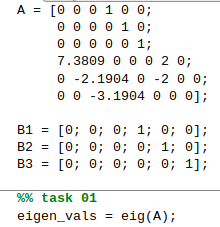
\includegraphics[width=0.3\textwidth]{task_01.png}
    \caption{matlab code 1}
\end{figure}

\section{Úkol 02}
Získal jsem matice řiditelnosti a zjistil jejich hodnosti, které postupně vyšly 4, 4, 2. Pro řiditelný 
systém bych potřeboval hodnost 6, takže ani s jedním samostatným vstupem není systém řiditelný.

\begin{figure}[h!]
    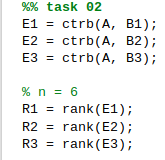
\includegraphics[width=0.2\textwidth]{task_02.png}
    \caption{matlab code 2}
\end{figure}

\section{Úkol 03}
Přenos jsem získal pomocí kódu na obrázku 3. Systém není řiditelný, protože v přenostu je vždy alespoň 
jeden řádek nulový.

\[
  H_1 = \begin{bmatrix}
  \frac{-(10000*(625*s^2 + 1369))}{(- 6250000*s^4 + 7440625*s^2 + 101044521)} \\
               \frac{(12500000*s)}{(- 6250000*s^4 + 7440625*s^2 + 101044521)} \\
                                                                    0 \\
\frac{-(10000*(625*s^3 + 1369*s))}{(- 6250000*s^4 + 7440625*s^2 + 101044521)} \\
             \frac{(12500000*s^2)}{(- 6250000*s^4 + 7440625*s^2 + 101044521) }\\
                                                                    0 \\
  \end{bmatrix}
\]

\[
H_2 = \begin{bmatrix}
                  \frac{-(12500000*s)}{(- 6250000*s^4 + 7440625*s^2 + 101044521)} \\
   \frac{-(625*(10000*s^2 - 73809))}{(- 6250000*s^4 + 7440625*s^2 + 101044521)} \\
                                                                      0 \\
              \frac{-(12500000*s^2)}{(- 6250000*s^4 + 7440625*s^2 + 101044521)} \\
\frac{(625*(- 10000*s^3 + 73809*s))}{(- 6250000*s^4 + 7440625*s^2 + 101044521)} \\
                                                                      0 \\
\end{bmatrix}
\]

\[
H_3 = \begin{bmatrix}
                       0 \\
                       0 \\
    \frac{625}{(625*s^2 + 1994)} \\
                       0 \\
                       0 \\
\frac{(625*s)}{(625*s^2 + 1994)} \\
\end{bmatrix}
\]

\begin{figure}[h!]
    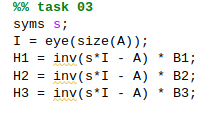
\includegraphics[width=0.2\textwidth]{task_03.png}
    \caption{matlab code 3}
\end{figure}

\newpage
\section{Úkol 04}

Zjistil jsem, že hodnost nové matice řiditelnosti je 7, což znamenená, že matice je řiditelná.

\begin{figure}[h!]
    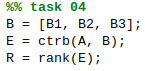
\includegraphics[width=0.2\textwidth]{task_04.png}
    \caption{matlab code 4}
\end{figure}

\section{Úkol 05}

Přenos spočítám pomocí kódu na obrázku, matice vyjde následovně:

\begin{equation*}
H = \begin{bmatrix}
  \frac{-(10000*(625s^2 + 1369))}{(- 6250000s^4 + 7440625s^2 + 101044521)} & \frac{-(12500000s)}{(- 6250000s^4 + 7440625s^2 + 101044521)} & 0 \\
  \frac{(12500000s)}{(- 6250000s^4 + 7440625s^2 + 101044521)} & \frac{-(625*(10000s^2 - 73809))}{(- 6250000s^4 + 7440625s^2 + 101044521)} & 0 \\
  0 & 0 & \frac{625}{(625s^2 + 1994)} \\
  \frac{-(10000*(625s^3 + 1369s))}{(- 6250000s^4 + 7440625s^2 + 101044521)} & \frac{-(12500000s^2)}{(- 6250000s^4 + 7440625s^2 + 101044521)} & 0 \\
  \frac{(12500000s^2)}{(- 6250000s^4 + 7440625s^2 + 101044521)} & \frac{(625*(- 10000s^3 + 73809s))}{(- 6250000s^4 + 7440625s^2 + 101044521)} & 0 \\
  0 & 0 & \frac{(625s)}{(625s^2 + 1994)} \\
\end{bmatrix}
\end{equation*}

Žádný řádek není nulový, takže matice je řiditelná.

\begin{figure}[h!]
    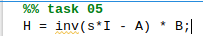
\includegraphics[width=0.2\textwidth]{task_05.png}
    \caption{matlab code 5}
\end{figure}

\end{document}